\documentclass[runningheads]{llncs}
%
\usepackage[T1]{fontenc}
% T1 fonts will be used to generate the final print and online PDFs,
% so please use T1 fonts in your manuscript whenever possible.
% Other font encondings may result in incorrect characters.
\usepackage{multirow}
\usepackage{multicol}
\usepackage{graphicx}
\usepackage{orcidlink}
%\usepackage{color}
%\renewcommand\UrlFont{\color{blue}\rmfamily}
%\usepackage[pagebackref=true,breaklinks=true,colorlinks,bookmarks=false]{hyperref}
%
\begin{document}
%
\title{Is Segment Anything Model a revolution in precision agriculture?}
%
%\titlerunning{Abbreviated paper title}
% If the paper title is too long for the running head, you can set
% an abbreviated paper title here
%

\author{
Alberto Carraro\inst{1}
\orcidlink{0000-0002-9747-0978}
\and
Francesco Marinello\inst{1}
%\orcidID{2222--3333-4444-5555}
}
\authorrunning{A. Carraro and F. Marinello}
% First names are abbreviated in the running head.
% If there are more than two authors, 'et al.' is used.
%
\institute{TESAF Department, University of Padova}
%
\maketitle              % typeset the header of the contribution
%
\begin{abstract}
Segment anything model (SAM) has revolutionized natural image segmentation, but its performance on medical images is limited. 
This work presents MedSAM, the first attempt at  extending the success of SAM to medical images, with the goal of creating a universal tool for the segmentation of various medical targets. 
Specifically, we first curate a large-scale medical image dataset, encompassing over 200,000 masks across 11 different modalities. Then, we develop a simple fine-tuning method to adapt SAM to general medical image segmentation. Comprehensive experiments on 21 3D segmentation tasks and 9 2D segmentation tasks demonstrate that MedSAM outperforms the default SAM model with an average Dice Similarity Coefficient (DSC) of 22.5\% and 17.6\% on 3D and 2D segmentation tasks, respectively.
The code and trained model are publicly available at \url{https://github.com/bowang-lab/MedSAM}.
\keywords{Segmentation Foundation Model \and Universal \and Multi-modality.}
\end{abstract}



\section{Introduction}
Medical image segmentation is a fundamental task in medical imaging analysis, which involves identifying and delineating regions of interest (ROI) in various medical images, such as organs, lesions, and tissues. Accurate segmentation is essential for many clinical applications, including disease diagnosis, treatment planning, and monitoring of disease progression. Deep learning-based models have shown great promise in medical image segmentation due to their ability to learn complex image features and provide accurate and efficient segmentation results. However, current models are often tailored to specific imaging modalities and targets, and their generalization ability is limited. Therefore, developing foundation models that can adapt to various medical imaging modalities and segmentation targets is of utmost importance in advancing medical image analysis.


Recently, segmentation foundation models have seen tremendous advancements in the field of natural image segmentation~\cite{2023-SAM-Meta}\cite{2023-SegGPT}\cite{2023-SEEM}, enabling accurate and efficient segmentation of objects in a fully automatic or interactive way. These models are typically based on transformer architectures and leverage pre-trained weights to achieve state-of-the-art performance and unprecedented generalization ability on a wide range of natural images. 

The first and the most well-known segmentation foundation model is the segment anything model~\cite{2023-SAM-Meta}, which is trained on more than 1 billion masks and has strong capabilities for generating accurate object masks based on prompts (e.g., bounding boxes, points, texts) or in a fully automatic manner. 
However, the applicability of these models to medical image segmentation remains limited due to the significant differences between natural images and medical images. Several studies have shown that SAM could fail on typical medical image segmentation tasks~\cite{SAM-pathology}, \cite{SAM-LiverTumor}, \cite{SAM-Meds}, \cite{SAM-DKFZ-Abdomen}, \cite{SAM-Polyps}, \cite{SAM-BrainMR}, \cite{SAM-Meds-2} and other challenging scenarios~\cite{SAM-Infrared},\cite{SAM-Camouflaged},\cite{SAM-Camouflaged2},\cite{SAM-RealworldApplication}, especially when the targets have weak boundaries. This is not surprising because SAM's training set mainly contains natural image datasets where the objects usually have strong edge information.

\begin{figure}[htbp]
\centering
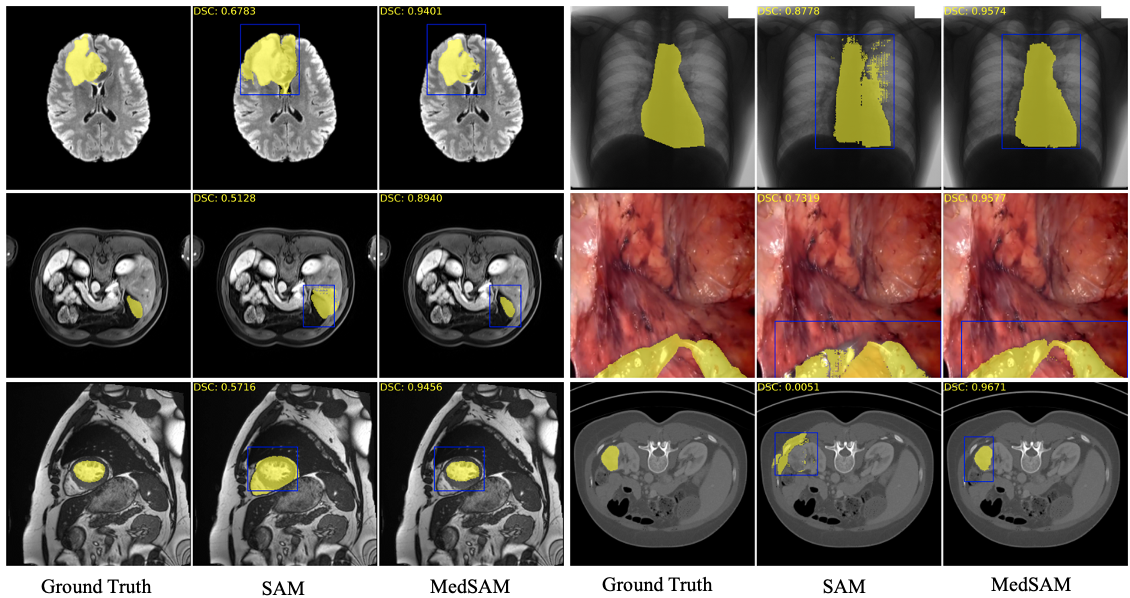
\includegraphics[scale=0.3]{imgs/fig1-seg-eg.png}
\caption{Visualized examples of the pre-trained SAM and MedSAM segmentation results. MedSAM significantly improves the segmentation performance across various modalities and segmentation tasks.}
\label{fig:sam-medsam}
\end{figure}

In this study, we introduce MedSAM for universal image segmentation, which is the first attempt at adapting SAM to the medical domain. Inspired by the success of SAM's strong capacity, primarily from large-scale supervised training, we first curate a diverse and comprehensive medical image dataset containing over 200,000 masks, spanning 11 medical image modalities. Next, we analyze the components of SAM's network architecture and assess their potential utility in medical image segmentation tasks. Finally, we develop a simple fine-tuning approach to adapt SAM to medical image segmentation. Our experiments on 21 3D image segmentation tasks and nine 2D image segmentation tasks demonstrate that our method can significantly improve SAM's performance on medical image segmentation tasks. 
% To facilitate further research in this promising area, we have made our code and trained models publicly available at \url{https://github.com/bowang-lab/MedSAM}.

\section{Methods}
\subsection{A teardown analysis of SAM}
The Segment Anything Model (SAM) utilizes a transformer-based architecture~\cite{attention-Nips17}, which has been shown to be highly effective in natural language processing~\cite{GPT-3} and image recognition tasks~\cite{ViT2020}. Specifically, SAM uses a vision transformer-based \textbf{image encoder} to extract image features and \textbf{prompt encoders} to incorporate user interactions, followed by a \textbf{mask decoder} to generate segmentation results and confidence scores based on the image embedding, prompt embedding, and output token. 

The vision transformer in the image encoder is pretrained with masked auto-encoder modeling~\cite{MAE}, which can process high-resolution images (i.e., 1024$\times$1024). The obtained image embedding is 16$\times$ downscaled (64$\times$64).
The prompt encoders are tailored for different user inputs. SAM supports four different prompts: points, boxes, texts, and masks. Each point is encoded by Fourier positional encoding~\cite{FourierPE-Nips20} and two learnable tokens for specifying foreground and background, respectively. The bounding box is encoded by the point encoding of its top-left corner and bottom-right corner. The free-form text is encoded by the pre-trained text-encoder in CLIP~\cite{CLIP-ICML2021}. The mask prompt has the same spatial resolution as the input image, which is encoded by convolution feature maps. 
Finally, the mask decoder employs a lightweight design, which consists of two transformer layers with a dynamic mask prediction head and an Intersection-over-Union (IoU) score regression head. The mask prediction head can generate three 4$\times$ downscaled masks, which correspond to the whole object, part, and subpart of the object, respectively.

\begin{figure}[h]
\centering
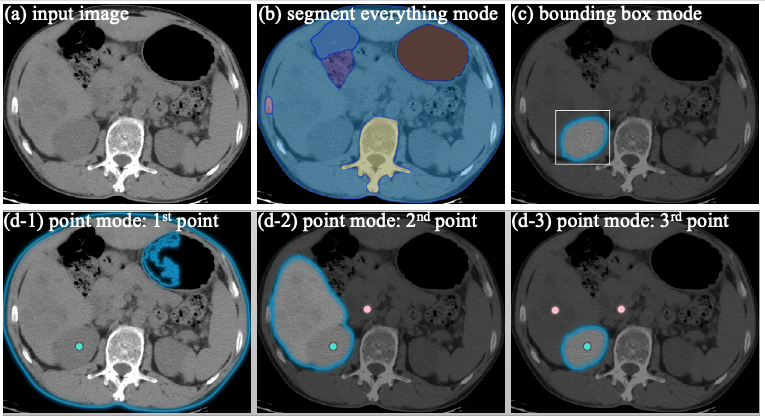
\includegraphics[scale=0.43]{imgs/fig2-SegModes.png}
\caption{Segmentation results of SAM based on different segmentation modes.}
\label{fig:sam-modes}
\end{figure}

\subsection{Understand SAM's utility from a medical perspective}
SAM supports three main segmentation modes: segmenting everything in a fully automatic way, bounding box mode, and point mode\footnote{Text prompts guided segmentation is not publicly available in SAM's official repository: \url{https://github.com/facebookresearch/segment-anything}.}. Fig.~\ref{fig:sam-modes} shows the results of the three segmentation modes on a typical abdominal Computed Tomography (CT) image\footnote{The results are based on the out-of-the-box online demo: \url{https://segment-anything.com/demo}}. The segment-everything mode divides the whole image into six regions based on the image intensity (Fig.~\ref{fig:sam-modes}b). However, such segmentation results have limited use because of two main reasons. On the one hand, the segmentation results do not have semantic labels.  On the other hand, clinicians mainly focus on meaningful ROIs in clinical scenarios, e.g., the liver, kidneys, spleen, and lesions. The bounding box-based segmentation mode generates good results for the right kidney by just giving the upper-left and bottom-right points (Fig.~\ref{fig:sam-modes}c). For the point-based segmentation mode (Fig.~\ref{fig:sam-modes}d), we first give one foreground point to the center of the right kidney but the segmentation results include the whole abdomen tissues. Then, we add a background point on the over-segmentation regions. The segmentation mask shrinks to the liver and right kidney. After adding another background point on the liver, we finally obtain the expected kidney segmentation.

To summarize, when applying SAM for medical image segmentation, the segment-everything mode is prone to generate useless region partitions and the point-based mode is ambiguous and requires multiple prediction-correction iterations. In contrast, the bounding box-based mode can clearly specify the ROI and obtain reasonable segmentation results without multiple trials and errors. In addition, one of the commonly used annotation methods is to label the longest diameter in radiology, e.g, the response evaluation criteria in solid tumors (RECIST)~\cite{RECIST09}. One can easily obtain the bounding box prompt of the target based on the RECIST annotation. Thus, we argue that the bounding box-based segmentation mode has wider practical values than the segment-everything and point-based mode when using SAM in medical image segmentation tasks.

\subsection{MedSAM: Dedicated medical image segmentation foundation models}
In order to adapt SAM for medical image segmentation, it is necessary to select an appropriate user prompt and the component of the network to fine-tune. 
Based on the above analysis, the bounding box prompt is a proper choice for specifying the segmentation target. SAM's network architecture contains three main components: image encoder, prompt encoder, and mask decoder. One can choose to fine-tune any of their combinations. The image encoder is based on a vision transformer, which has the maximum computational overhead in SAM. 
To minimize computation costs, we keep the image encoder frozen. 
The prompt encoder encodes the positional information of the bounding box and can be reused from the pre-trained bounding-box encoder in SAM, so we also freeze this component. The remaining part that requires fine-tuning is the mask decoder, as illustrated in Fig.~\ref{fig:medsam}. 

\begin{figure}[htbp]
\centering
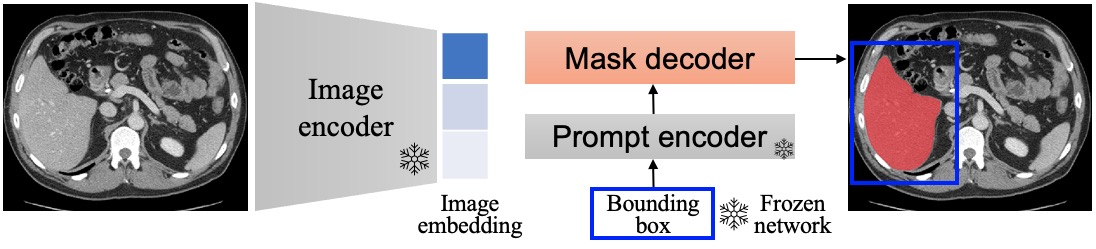
\includegraphics[scale=0.3]{imgs/fig3-MedSAM.png}
\caption{MedSAM: fine-tuning SAM for medical image segmentation. We freeze the image encoder and prompt encoder and only fine-tune the mask decoder.}
\label{fig:medsam}
\end{figure}

Since the image encoder can be applied prior to prompting the model, we can pre-compute the image embedding for all training images to avoid replicated computing of the image embedding per prompt, which can significantly improve the training efficiency. The mask decoder only needs to generate one mask rather than three masks because the bounding box prompt can clearly specify the expected segmentation target in most situations. 


\section{Experiments and Results}
\subsection{Data curation and preprocessing}
We curated a large-scale and diverse dataset with 33 segmentation tasks, including brain ventricle, brain tumor, cerebellum, gallbladder, heart left and right ventricle, liver, pancreas, and prostate segmentation in various MR sequences (e.g., T1, T2, ADC, FLAIR)~\cite{AMOS22}\cite{MMs2020}\cite{ACDC}\cite{ABCs-MICCAI20}\cite{bakas2018brats}\cite{nci_prostate_dataset}\cite{PROMISE12}\cite{MSD-Dataset}, abdomen tumor, COVID-19 infection, gallbladder, head and neck tumor, liver, pancreas, pleural effusion, and stomach segmentation in CT images~\cite{Ma-2020-abdomenCT-1K}\cite{KiTS2021MIA}\cite{LiTS}\cite{FLARE21-MIA}\cite{ma2021-COVID-Data}\cite{MSD-Dataset}\cite{HECKTOR2021overview}\cite{NSCLC1}\cite{NSCLC2}\cite{TCIA}, breast tumor, liver, and vessel segmentation in ultrasound images~\cite{BUSIDataset}\cite{US-abdomen-data}, heart and lungs segmentation in X-Ray images~\cite{XRay-JSRT}, polyp and instrument segmentation in endoscope images~\cite{polyp-nature-data}\cite{Endo-instrument}, vessel segmentation in retinal images~\cite{DRIVE}, and colon gland segmentation in pathology images~\cite{gland-patho1}\cite{gland-patho2}.

For medical images, intensity values can span a wide range. To facilitate stable training, we normalized all images to the same intensity range. For CT images, we clipped the intensity values to the range [-500, 1000], as this range encompasses most tissues. For other images, we clipped the intensity values to the range between the 0.95th and 99.5th percentiles. We then normalized all intensity values to the range [0, 255] and resized the images to a uniform size of 256 $\times$ 256 $\times$ 3.


\subsection{Training protocol}
Each dataset was randomly split into 80 and 20 for training and testing. The segmentation targets with fewer than 100 pixels were excluded. Since SAM is designed for 2D image segmentation, we divided 3D images (i.e., CT, MR, PET) into 2D slices along the out-of-plane dimension. 
Then, we used the pre-trained ViT-Base model as the image encoder and computed all the image embedding offline by feeding the normalized images to the image encoder (the image encoder will transform the image size to 3 $\times$ 1024 $\times$ 1024).
During training, the bounding box prompt was generated from the ground-truth mask with a random perturbation of 0-20 pixels. 
The loss function is the unweighted sum between Dice loss and cross-entropy loss, which has been proven to be robust in various segmentation tasks~\cite{nnunet21}\cite{SegLossOdyssey}. The network was optimized by Adam~\cite{ADAM15} optimizer with an initial learning rate of 1e-5.

\subsection{Evaluation results on 21 3D image segmentation tasks and 9 2D image segmentation tasks}
We used the Dice Similarity Coefficient (DSC) and Normalized Surface Distance (NSD, tolerance 1 $mm$) to evaluate the region overlap ratio and boundary consensus between the ground truth and segmentation results, which are two commonly used segmentation metrics~\cite{metric-reload}. Table~\ref{tab:3d} and Table~\ref{tab:2d} present the quantitative comparison between the pretrained SAM (ViT-B) model and our MedSAM on 21 3D image segmentation tasks and 9 2D image segmentation tasks. It can be found that MedSAM achieved remarkable improvements across all 30 segmentation tasks, with an improved average DSC of 22.5\% and NSD of 39.1\% on 3D image segmentation tasks and DSC of 17.6\% and NSD of 18.9\% on 2D image segmentation tasks. 

% Fig. 4 visualizes the performance distribution of the pretrained SAM and MedSAM on different tasks. 
The pre-trained SAM model shows good performance for large-organ segmentation tasks, such as the cerebellum and liver segmentation, but yields poor results for lesion segmentation tasks, for example, the abdomen tumor, lung COVID-19 infections, and pleural effusion segmentation. Additionally, the pre-trained SAM struggles to generate consistent boundaries on all 3D tasks, resulting in low NSD scores. Conversely, for 2D tasks, the pre-trained SAM exhibits comparable average DSC scores, but better NSD scores. This is because segmentation targets often have more well-defined boundaries in 2D images, such as the instrument in endoscope videos. In contrast, our MedSAM model outperforms the pre-trained SAM model by a significant margin in both DSC and NSD scores across all tasks.


We also present more segmentation examples in Fig.~\ref{fig:medsam2}. The pre-trained SAM model is particularly susceptible to producing over-segmentation results, making it challenging to accurately segment targets with weak boundaries. For instance, the pre-trained SAM failed to provide accurate segmentation results for lesions in ultrasound and MR images, even with a relatively tight bounding box prompt. Furthermore, when the content inside the bounding box is heterogeneous, the model may not identify the correct segmentation target. Additionally, when segmenting targets with clear boundaries, SAM may generate outliers when the surrounding objects also have good contrasts, as seen in the instrument segmentation in endoscope images.


Through the fine-tuning of SAM on medical image datasets, MedSAM has greatly enhanced the model's ability to identify challenging segmentation targets. Specifically, MedSAM has demonstrated three significant improvements over the pre-trained SAM. Firstly, MedSAM has improved the model's ability to identify small objects, even when multiple segmentation targets are present within the bounding box prompt. Secondly, the model has shown more robustness towards weak boundaries in various modalities, such as lesion and left ventricle segmentation in ultrasound and brain MR images, respectively. Finally, MedSAM has effectively reduced interference from high-contrast objects surrounding the segmentation target, resulting in fewer outliers.

% 21 tasks
% Please add the following required packages to your document preamble:
% \usepackage{multirow}
\begin{table}[]
\caption{Performance comparison between MedSAM and SAM on 21 3D medical image segmentation tasks. MedSAM achieves significant and consistent improvements across all the tasks.}\label{tab:3d}
\centering
\begin{tabular}{llccc|ccc}
\hline
\multirow{2}{*}{Segmentation Target} & \multirow{2}{*}{Modality} & \multicolumn{3}{c|}{DSC (\%)}              & \multicolumn{3}{c}{NSD (\%)}              \\ \cline{3-8} 
                                     &                           & MedSAM  & SAM     & Improve     & MedSAM  & SAM     & Improve     \\ \hline
Brain Ventricles                     & MR-T1                     & 74.82 & 41.96 & \textbf{32.86} & 78.17 & 31.26 & \textbf{46.91} \\
Brain Ventricles                     & MR-T2                     & 72.87 & 39.56 & \textbf{33.31} & 75.01 & 31.39 & \textbf{43.62} \\
Brain Tumor                          & MR-FLAIR                  & 89.15 & 74.00 & \textbf{15.15} & 76.13 & 38.27 & \textbf{37.86} \\
Cerebellum                           & MR-T1                     & 93.31 & 83.25 & \textbf{10.06} & 82.39 & 44.55 & \textbf{37.84} \\
Cerebellum                           & MR-T2                     & 90.78 & 81.88 & \textbf{8.90}  & 70.01 & 38.84 & \textbf{31.17} \\
Gallbladder                          & MR                        & 77.78 & 61.97 & \textbf{15.81} & 76.36 & 36.34 & \textbf{40.02} \\
Left Ventricle                 & MR                        & 88.91 & 68.44 & \textbf{20.48} & 91.05 & 55.73 & \textbf{35.32} \\
Right Ventricle                & MR                        & 85.92 & 72.11 & \textbf{13.80} & 88.85 & 68.98 & \textbf{19.87} \\
Liver                                & MR                        & 93.90 & 80.38 & \textbf{13.52} & 80.13 & 33.00 & \textbf{47.13} \\
Pancreas                             & MR                        & 80.07 & 51.11 & \textbf{28.96} & 79.42 & 32.81 & \textbf{46.61} \\
Prostate                             & MR-ADC                    & 92.25 & 79.61 & \textbf{12.65} & 92.72 & 60.12 & \textbf{32.59} \\
Prostate                             & MR-T2                     & 92.18 & 79.39 & \textbf{12.78} & 92.00 & 57.60 & \textbf{34.40} \\
Abdomen Tumor                        & CT                        & 65.54 & 42.86 & \textbf{22.68} & 64.99 & 34.49 & \textbf{30.50} \\
Gallbladder                          & CT                        & 84.36 & 47.28 & \textbf{37.08} & 87.07 & 30.48 & \textbf{56.59} \\
Head-Neck Tumor                      & CT                        & 68.29 & 23.87 & \textbf{44.41} & 47.36 & 23.88 & \textbf{23.48} \\
Liver                                & CT                        & 91.42 & 74.21 & \textbf{17.21} & 76.30 & 26.08 & \textbf{50.21} \\
Lung Infections                      & CT                        & 60.01 & 32.54 & \textbf{27.47} & 58.89 & 25.84 & \textbf{33.04} \\
Pancreas                             & CT                        & 76.76 & 43.53 & \textbf{33.23} & 81.09 & 32.38 & \textbf{48.71} \\
Pleural Effusion                     & CT                        & 59.46 & 9.52  & \textbf{49.94} & 75.77 & 11.19 & \textbf{64.59} \\
Stomach                              & CT                        & 82.66 & 68.95 & \textbf{13.72} & 70.93 & 35.49 & \textbf{35.44} \\
Head-Neck Tumor                      & PET                       & 81.17 & 72.45 & \textbf{8.72}  & 62.76 & 38.57 & \textbf{24.18} \\ \hline
\multicolumn{2}{c}{Average}                                      & 81.04 & 58.52 & \textbf{22.51} & 76.57 & 37.51 & \textbf{39.05} \\ \hline
\end{tabular}
\end{table}


% 9 tasks
\begin{table}[]
\caption{Performance comparison between MedSAM and SAM on nine 2D medical image segmentation tasks. MedSAM achieves significant and consistent improvements across all the tasks.}\label{tab:2d}
\centering
\begin{tabular}{llccc|ccc}
\hline
\multirow{2}{*}{Segmentation Target} & \multirow{2}{*}{Modality} & \multicolumn{3}{c|}{DSC (\%)}             & \multicolumn{3}{c}{NSD (\%)}              \\ \cline{3-8} 
                                     &                           & MedSAM  & SAM     & Improve     & MedSAM  & SAM     & Improve     \\ \hline
Breast Tumor                         & Ultrasound                & 85.42 & 78.01 & \textbf{7.41}  & 89.02 & 82.48 & \textbf{6.54}  \\
Liver                                & Ultrasound                & 74.36 & 67.81 & \textbf{6.55}  & 79.07 & 72.07 & \textbf{7.01}  \\
Vessel                               & Ultrasound                & 70.88 & 57.60 & \textbf{13.28} & 78.41 & 65.10 & \textbf{13.31} \\
Heart                                & X-Ray                     & 91.19 & 79.28 & \textbf{11.91} & 94.10 & 83.85 & \textbf{10.25} \\
Lungs                                & X-Ray                     & 96.57 & 72.24 & \textbf{24.33} & 98.56 & 75.45 & \textbf{23.11} \\
Polyp                                & Endoscope                 & 86.90 & 81.60 & \textbf{5.30}  & 90.91 & 85.93 & \textbf{4.99}  \\
Instrument                           & Endoscope                 & 86.37 & 76.61 & \textbf{9.76}  & 90.93 & 82.36 & \textbf{8.57}  \\
Retinal Vessel                       & Retinal Image             & 66.10 & 0.75  & \textbf{65.35} & 84.40 & 3.45  & \textbf{80.95} \\
Gland                                & Pathology                 & 37.23 & 22.63 & \textbf{14.60} & 43.09 & 27.75 & \textbf{15.33} \\ \hline
\multicolumn{2}{c}{Average}                                      & 77.22 & 59.62 & \textbf{17.61} & 83.17 & 64.27 & \textbf{18.89} \\ \hline
\end{tabular}
\end{table}


\begin{figure}[htbp]
\centering
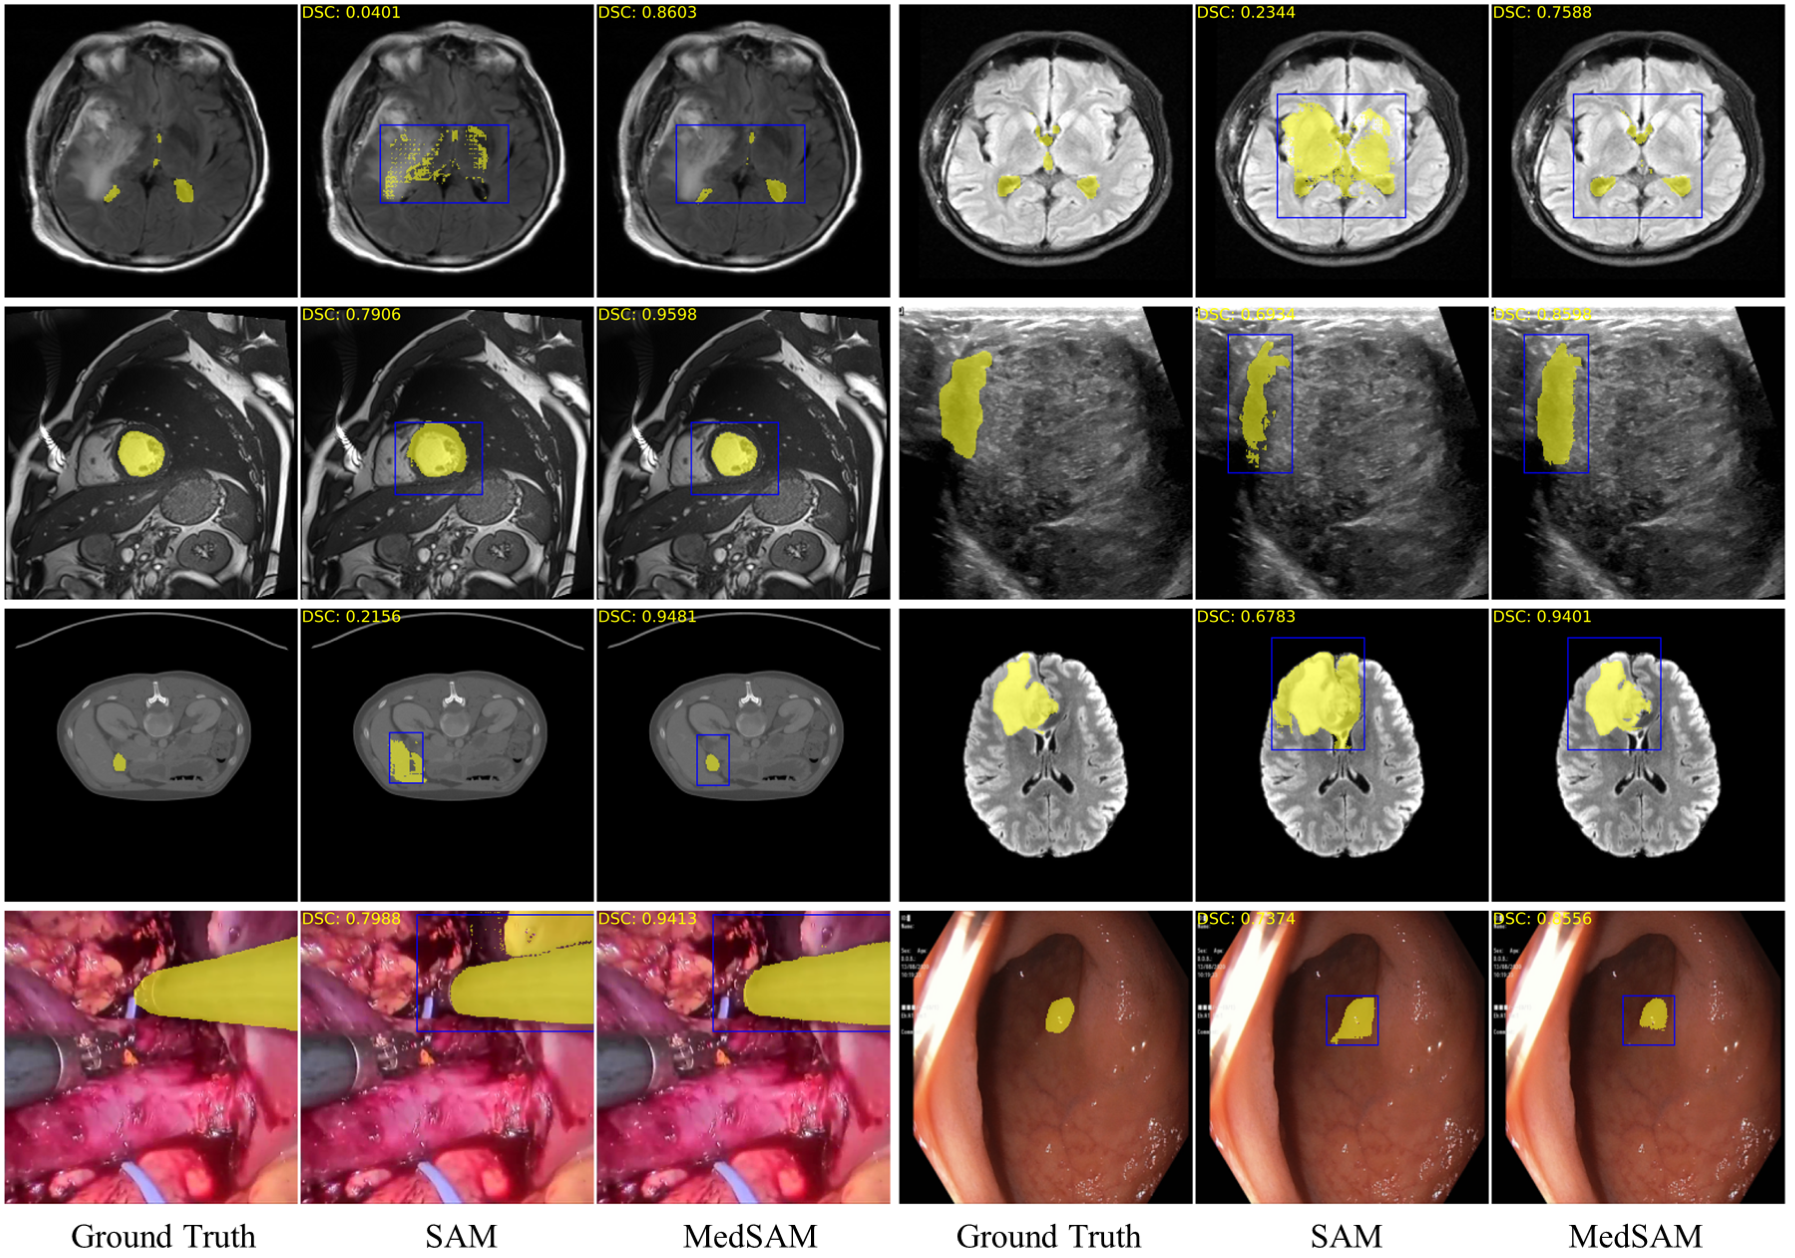
\includegraphics[scale=0.41]{imgs/fig5-MedSAM-Res2.png}
\caption{More examples of the pre-trained SAM and MedSAM on different 3D and 2D medical image segmentation tasks.}
\label{fig:medsam2}
\end{figure}

% \subsection{Future work}
% 




% multi-mask output could be useful in some nested segmentation tasks, brain tumor
\section{Discussion and Conclusion}
We have shown that fine-tuning the mask encoder can lead to significant improvements in various segmentation tasks and image modalities. However, its overall performance still lags behind specialist models, such as those developed for liver segmentation in abdomen CT images~\cite{FLARE21-MIA} and left and right ventricle segmentation in heart MR images~\cite{MMs2020}, particularly in terms of boundary consensus. There is also considerable room for improvement in lesion segmentation tasks, including abdomen tumor and lung COVID-19 infections segmentation.

\begin{figure}[htbp]
\centering
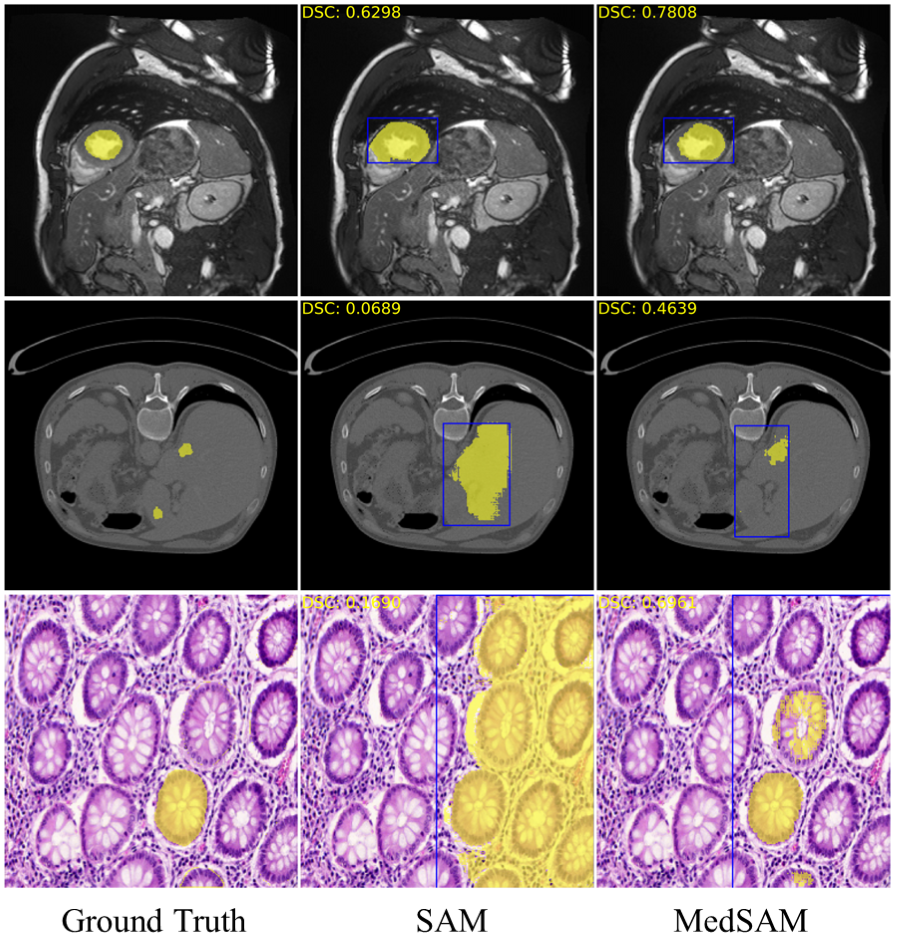
\includegraphics[scale=0.8]{imgs/fig6-bad-seg.png}
\caption{Failure case analysis. The model suffers from objects with missing boundaries, low contrast, and tiny size. Moreover, over loose bounding box could lead to inaccurate segmentation if there are many similar objects inside the bounding box.}
\label{fig:failed}
\end{figure}

Several failure cases are presented in Fig.~\ref{fig:failed}. The pre-trained SAM and MedSAM both have limited ability to handle objects with missed boundaries, as seen in the over-segmentation results of left ventricle segmentation in heart MR images. The models could also miss tiny and low-contrast objects inside the bounding box, such as in the liver tumor segmentation in abdomen CT images. Additionally, if multiple similar instances surround the segmentation target, a large bounding box may introduce incorrect segmentation results, such as in the gland segmentation in pathology images.

We anticipate that the limitations of MedSAM could be overcome by leveraging larger models and increasing the dataset size. In our study, we used the smallest image encoder (ViT-base) and did not fine-tune the image encoder to reduce the computing burden. By using larger backbone models and fine-tuning the image encoder, the model capacity can be further improved and learn more medical image features. While our training set contains more than 200,000 masks, it is still relatively small compared to SAM's training set. The data ablation studies in SAM show that the model's performance with one million images is comparable to the model with 11 million images~\cite{2023-SAM-Meta}. Therefore, a training set with one million images (approximately 100 million masks) would be a reasonable scale for the training set. In the future, we plan to expand our training set to this scale to further improve MedSAM's performance.


In addition to the bounding box, scribble is another commonly used user interaction in medical image segmentation~\cite{wang-deepigeos-PAMI}\cite{wang-interactive2}, which was not supported in the current SAM. This interaction is not only simple and efficient but also to be quite useful for some non-compact targets, such as myocardium segmentation. 
Therefore, we plan to incorporate the scribble-based prompt into the MedSAM, which can be combined with the bounding box prompt for various segmentation tasks, further improving the model's segmentation accuracy. Additionally, integrating MedSAM into commonly used medical image viewers, such as 3D slicer~\cite{SAM-3DSlicer} and Napari\footnote{\url{https://github.com/MIC-DKFZ/napari-sam}}, will enable more end-users to access state-of-the-art models without requiring extensive coding knowledge.

In conclusion, the success of SAM on natural images demonstrates the feasibility of building segmentation foundation models. This work presents the first attempt to adapt SAM to medical image segmentation by fine-tuning the pre-trained model on medical image datasets. We have achieved remarkable performance improvements across a wide range of tasks and image modalities. We hope this work will motivate more studies to build segmentation foundation models in the medical image domain, and we anticipate that the field will experience a GPT-4 moment in the near future. Our code and trained model are publicly available, and we provide a step-by-step tutorial on fine-tuning SAM on customized new datasets. 
Our code and trained model have been publicly available and we also provide a step-by-step tutorial on fine-tuning SAM on customized new datasets. 
We look forward to working with the community together to advance this exciting research area.



\subsubsection{Acknowledgements} 
The authors of this paper highly appreciate all the challenge organizers and owners for providing the public dataset to the community. We also thank Meta AI for making the source code of segment anything publicly available to the community. 

% ---- Bibliography ----
%
% BibTeX users should specify bibliography style 'splncs04'.
% References will then be sorted and formatted in the correct style.
\newpage
\bibliographystyle{splncs04}
\bibliography{ref}

\end{document}
